\subsection{Vereinzelung} \label{sec:Vereinzelung}
\textit{(ygu)} Die Umsetzung der Vereinzelung orientiert sich stark am realisierten Funktionsnachweis. Der grundlegende Aufbau wurde beibehalten. Hinzu kommen einige Erweiterungen, um die Zuverlässigkeit zu steigern sowie Verbesserungen in der Benutzerfreundlichkeit zu erreichen.
\newline

\textbf{Aufbau und Funktion}
\newline
Die Vereinzelung besteht aus einer Trommel (Punkt. 1 in Abbildung \ref{fig:details_vereinzelung}), worin die NemaCaps eingefüllt werden. Durch die Rotation der Lochmaske (3), welche durch einen Getriebemotor (7) umgesetzt wird, fallen die NemaCaps in die vorgesehenen Löcher. Überschüssige NemaCaps werden durch mehrere Bürsten (6) abgestreift. Sobald die vereinzelten NemaCaps bei den Schlauchkupplungen (8) angekommen sind, sollen diese durch die Schläuche zur Einsetzlokalität fallen. Alle Komponenten werden auf einer Grundplatte (4) montiert, wobei diese in ihrer Neigung verstellbar gelagert ist.
	\begin{figure}[H]
	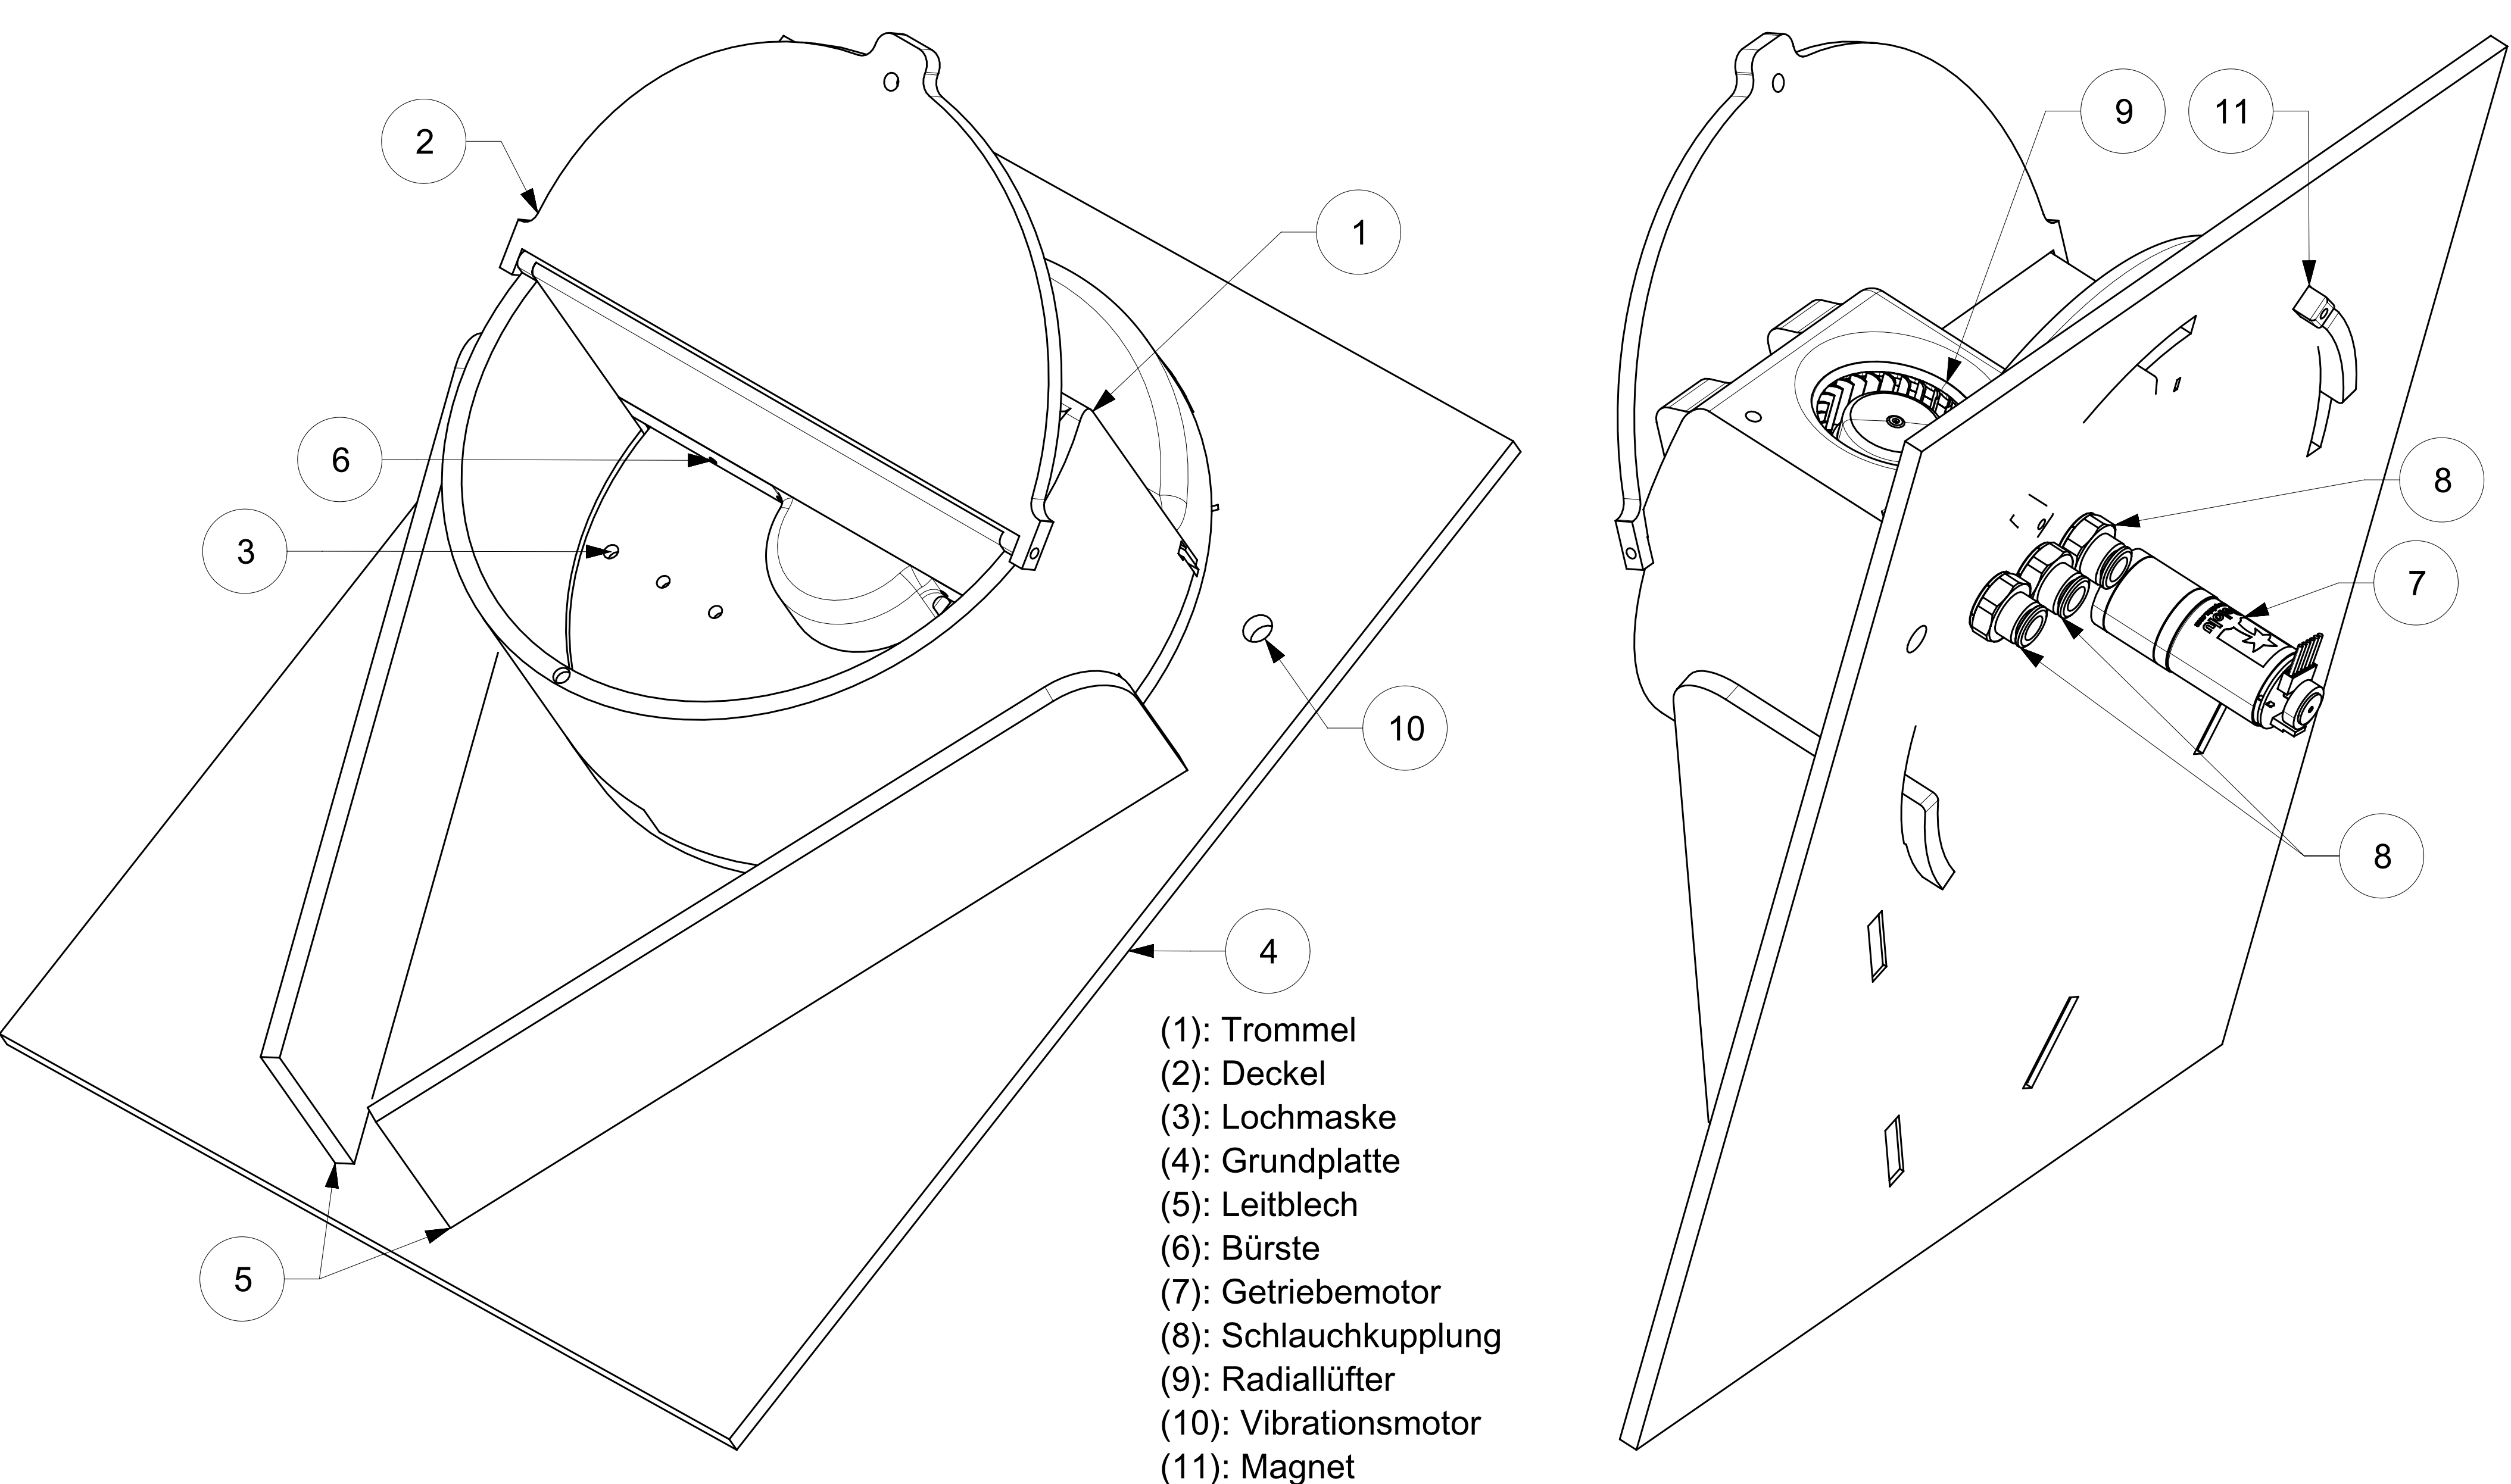
\includegraphics[scale=0.455]{Illustrationen/6-Umsetzung/details_vereinzelung.jpg}
	\caption{Detaillierte Übersicht der Vereinzelung}
	\label{fig:details_vereinzelung}
	\end{figure}
\newpage
\textbf{Abhilfemassnahmen}
\newline
Der Funktionsnachweis aus Kapitel \ref{funktionsnachweis} zeigte auf, dass Komplikationen auftretten können. In erschwerten Bedingungen, wie nassem Pulver, kann das NemaCap  durch die erhöhte Adhäsion an der Lochmaske hängen bleiben. So wurde im Funktionsnachweis die Bedingung formuliert, dass eine Umsetzung dieser Funktion nur mit konkreten Abhilfemassnahmen umgesetzt werden darf, um die Zuverlässigkeit der Vereinzelung zu steigern. Diese sind:
\begin{itemize}
	\item \textbf{Vibrationsmotor:} Der Funktionsnachweis zeigte, dass durch leichtes Klopfen an der Einheit, hängengebliebene NemaCaps erfolgreich gelöst werden. Somit wird in der Nähe der Schlauchkupplungen ein Vibrationsmotor (Punkt. 10 in Abbildung \ref{fig:details_vereinzelung}) angebracht, welche die Einheit in Schwingung bringen soll. Wichtig ist dabei, dass die Grundplatte in eine Richtung federnd gelagert wird, sodass diese tatsächlich in Schwingung geraten kann.
	
	\item \textbf{Radiallüfter:} Eine weitere Möglichkeit die NemaCaps zu lösen, bietet ein gezielter Luftstoss. Daher ist in der Trommel ein Radiallüfter (9) integriert, welcher einen Luftstrom auf die vereinzelten NemaCaps in der Lochmaske richtet. Bei Bedarf werden zusätzliche Löcher an den Schläuchen angebracht, um den Luftaustritt zu verbessern. 
	
	\item \textbf{Lochmaske:} Am Funktionsnachweis wurde ersichtlich, wie kritisch die Materialwahl sowie Fertigungsqualität der Lochmaske ist. Die formulierten Punkte zur Steigerung der Zuverlässigkeit sind in diesem Kapitel unter \textit{Lochmaske} \textbf{(anders markieren?)} erläutert.
\end{itemize}

\textbf{Handhabung}
\newline
Die Verwendung von frischen NemaCaps und somit frischem Pulver trägt zur verbesserten Zuverlässigkeit der Vereinzelung bei. Der benutzerfreundliche Wechsel von NemaCaps ist also ein wichtiges Anliegen und ist in der Konstruktion der Vereinzelung berücksichtigt. So ist die Trommel (Punkt 1 in Abb. \ref{fig:vereinzelung_entleeren}) mit einem dreifachen Bajonettverschluss (Detail C, 12) versehen. Die Trommel kann mit einer Drehung von 15° im Gegenuhrzeigersinn entriegelt werden (Detail A in Abb. \ref{fig:vereinzelung_entleeren}). Nun kann die Trommel entfernt werden (Detail B). Die verbleibenden NemaCaps (Detail X) rollen nun auf der Grundplatte hinunter. Gelenkt durch zwei Leitbleche (5) fallen diese in Richtung Detail Y, wo man diese in einem Behälter sammeln kann. Auch verfügt die Trommel über einen Deckel (2), welcher durch zwei angebrachte Magnete sicher verschlossen wird.
	\begin{figure}[H]
	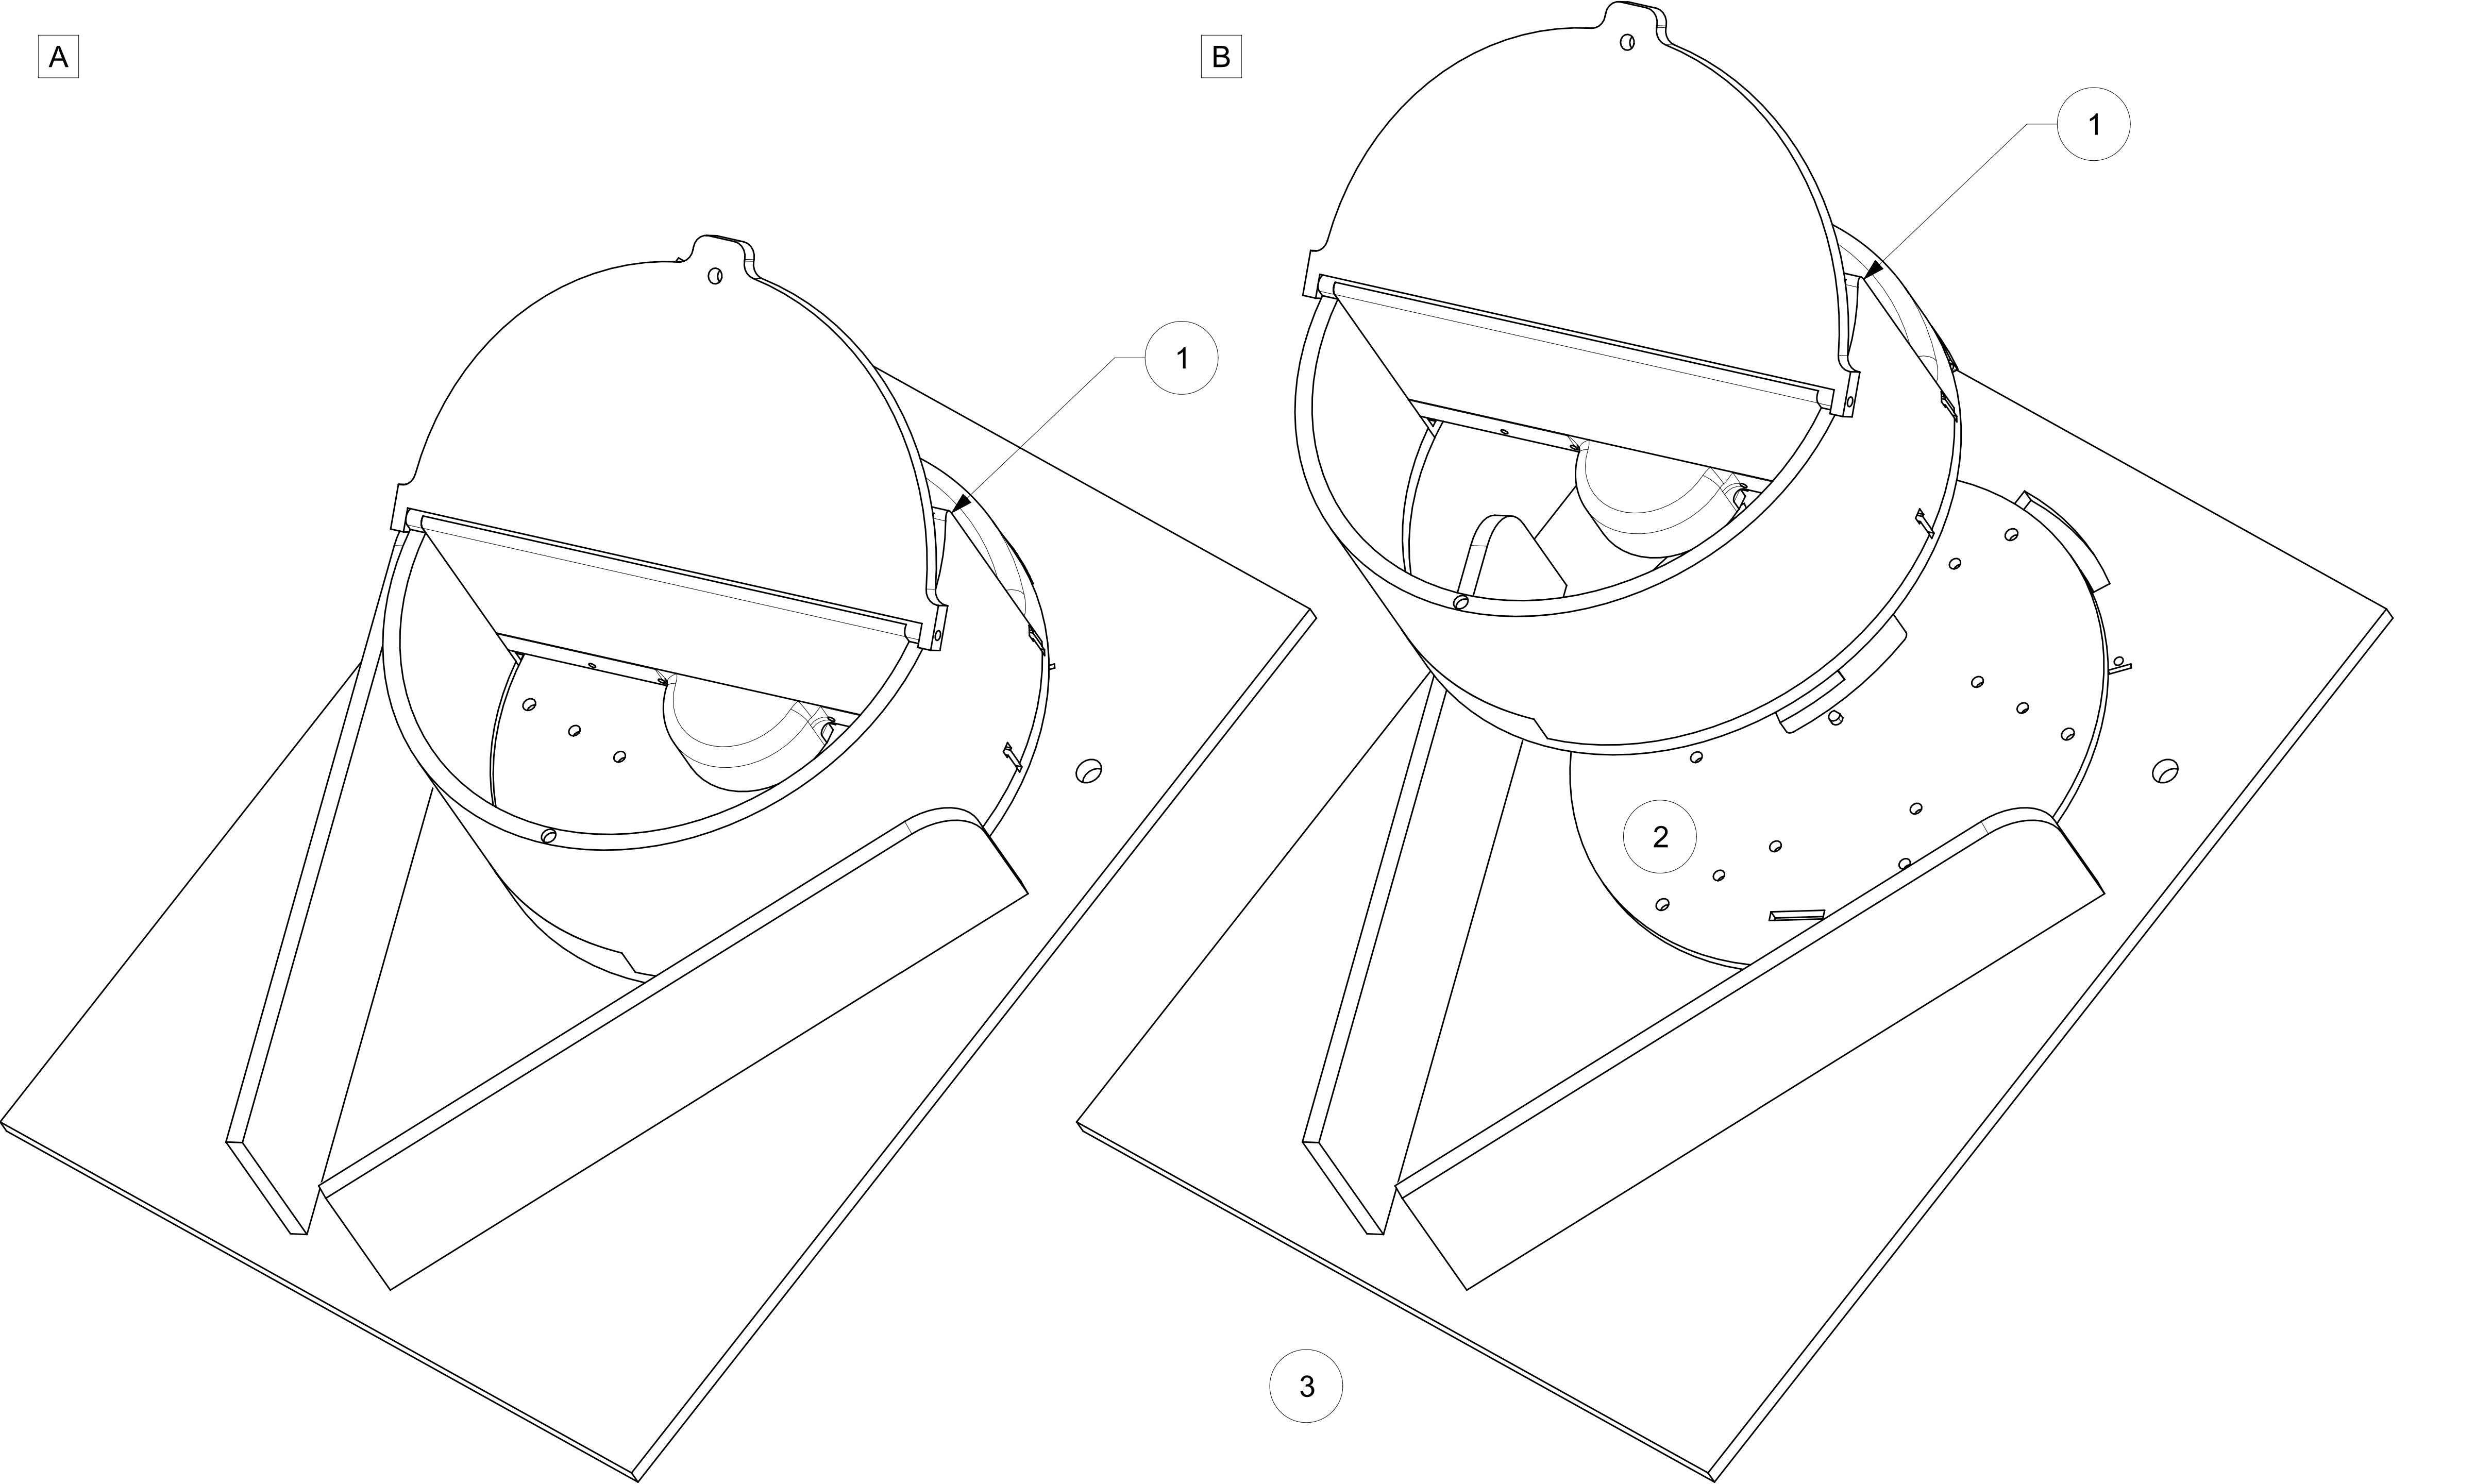
\includegraphics[scale=0.42]{Illustrationen/6-Umsetzung/vereinzelung_entleeren.jpg}
	\caption{Entleerung der Trommel}
	\label{fig:vereinzelung_entleeren}
	\end{figure}
\textbf{Lochmaske}
\newline
Der Funktionsnachweis hat gezeigt, dass das Scheitern der Vereinzelung meist durch das Hängenbleiben der NemaCaps an der Lochmaske verursacht wird. Die Zuverlässigkeit dieser Funktion hängt direkt von den Eigenschaften der Lochmaske ab. Die Materialwahl sowie Fertigungsqualität von diesem Teil ist entscheidend. 
\newline
Folgende Massnahmen werden umgesetzt:
\begin{itemize}
	\item \textbf{Materialwahl:} Die Wahl des passenden Materials mit der geringsten Adhäsion wurde mittels praktischen Tests am 26.4.2017 durchgeführt. Dabei wurden gängige laserbare Materialien (Aluminium, Plexiglas und MDF) miteinander verglichen. Die Tests zeigen, dass Aluminium die geringste Adhäsion gegenüber von NemaCaps aufweist, gefolgt von Plexiglas. Mit MDF wurde die grösste Adhäsion festgestellt, was durch die erhöhte Pulveraufnahme sowie die rauhere Oberfläche zu erklären ist. 
	Die höchste Zufriedenstellung wird mit Aluminium erreicht, wobei die Reibung zwischen Lochmaske und Grundplatte noch nicht berücksichtigt ist. Bei zu hoher Reibung kann auf Plexiglas ausgewichen werden.
	
	\item \textbf{Fertigungsqualität:} Die Tests vom 26.4.2017 zeigten auch, dass die Rauheit der Oberfläche relevant ist. Je feiner die Oberfläche der Bohrung (Punkt 13 in Abbildung \ref{fig:detail_lochmaske}), desto geringer ist das Risiko, dass NemaCaps hängenbleiben. Somit werden diese Löcher nach der Bohrung zusätzlich mit einer Reibale (\textbf{H7?}) ausgerieben. Der ideale Durchmesser D1 muss während der Inbetriebnahme durch zielgerichtetes Ausprobieren erörtert werden.
	
	\item \textbf{Fertigungsverfahren:} Gegeben durch den einfachen zweidimensionalen Aufbau wird die Lochmaske \textbf{mit dem Laser hergsetellt (korrekt?)}. Als Dicke bietet sich 4mm an, sodass ein grosses NemaCap Platz findet und weitere abgestreift werden.
\end{itemize}
Desweiteren ist die Lochmaske mit zwei Langlöchern (14) ausgestattet. Diese werden zur Einpassung von Dauermagneten verwendet, welche zur Positionsbestimmung der Lochmaske dienen. Konstruktiv ist hinzuzufügen, dass der Abstand B in Abbildung \ref{fig:detail_lochmaske} gegeben ist durch die Dimensionen der Schlauchkupplungen (Punkt 8 in Abb. \ref{fig:details_vereinzelung}).
	\begin{figure}[H]
	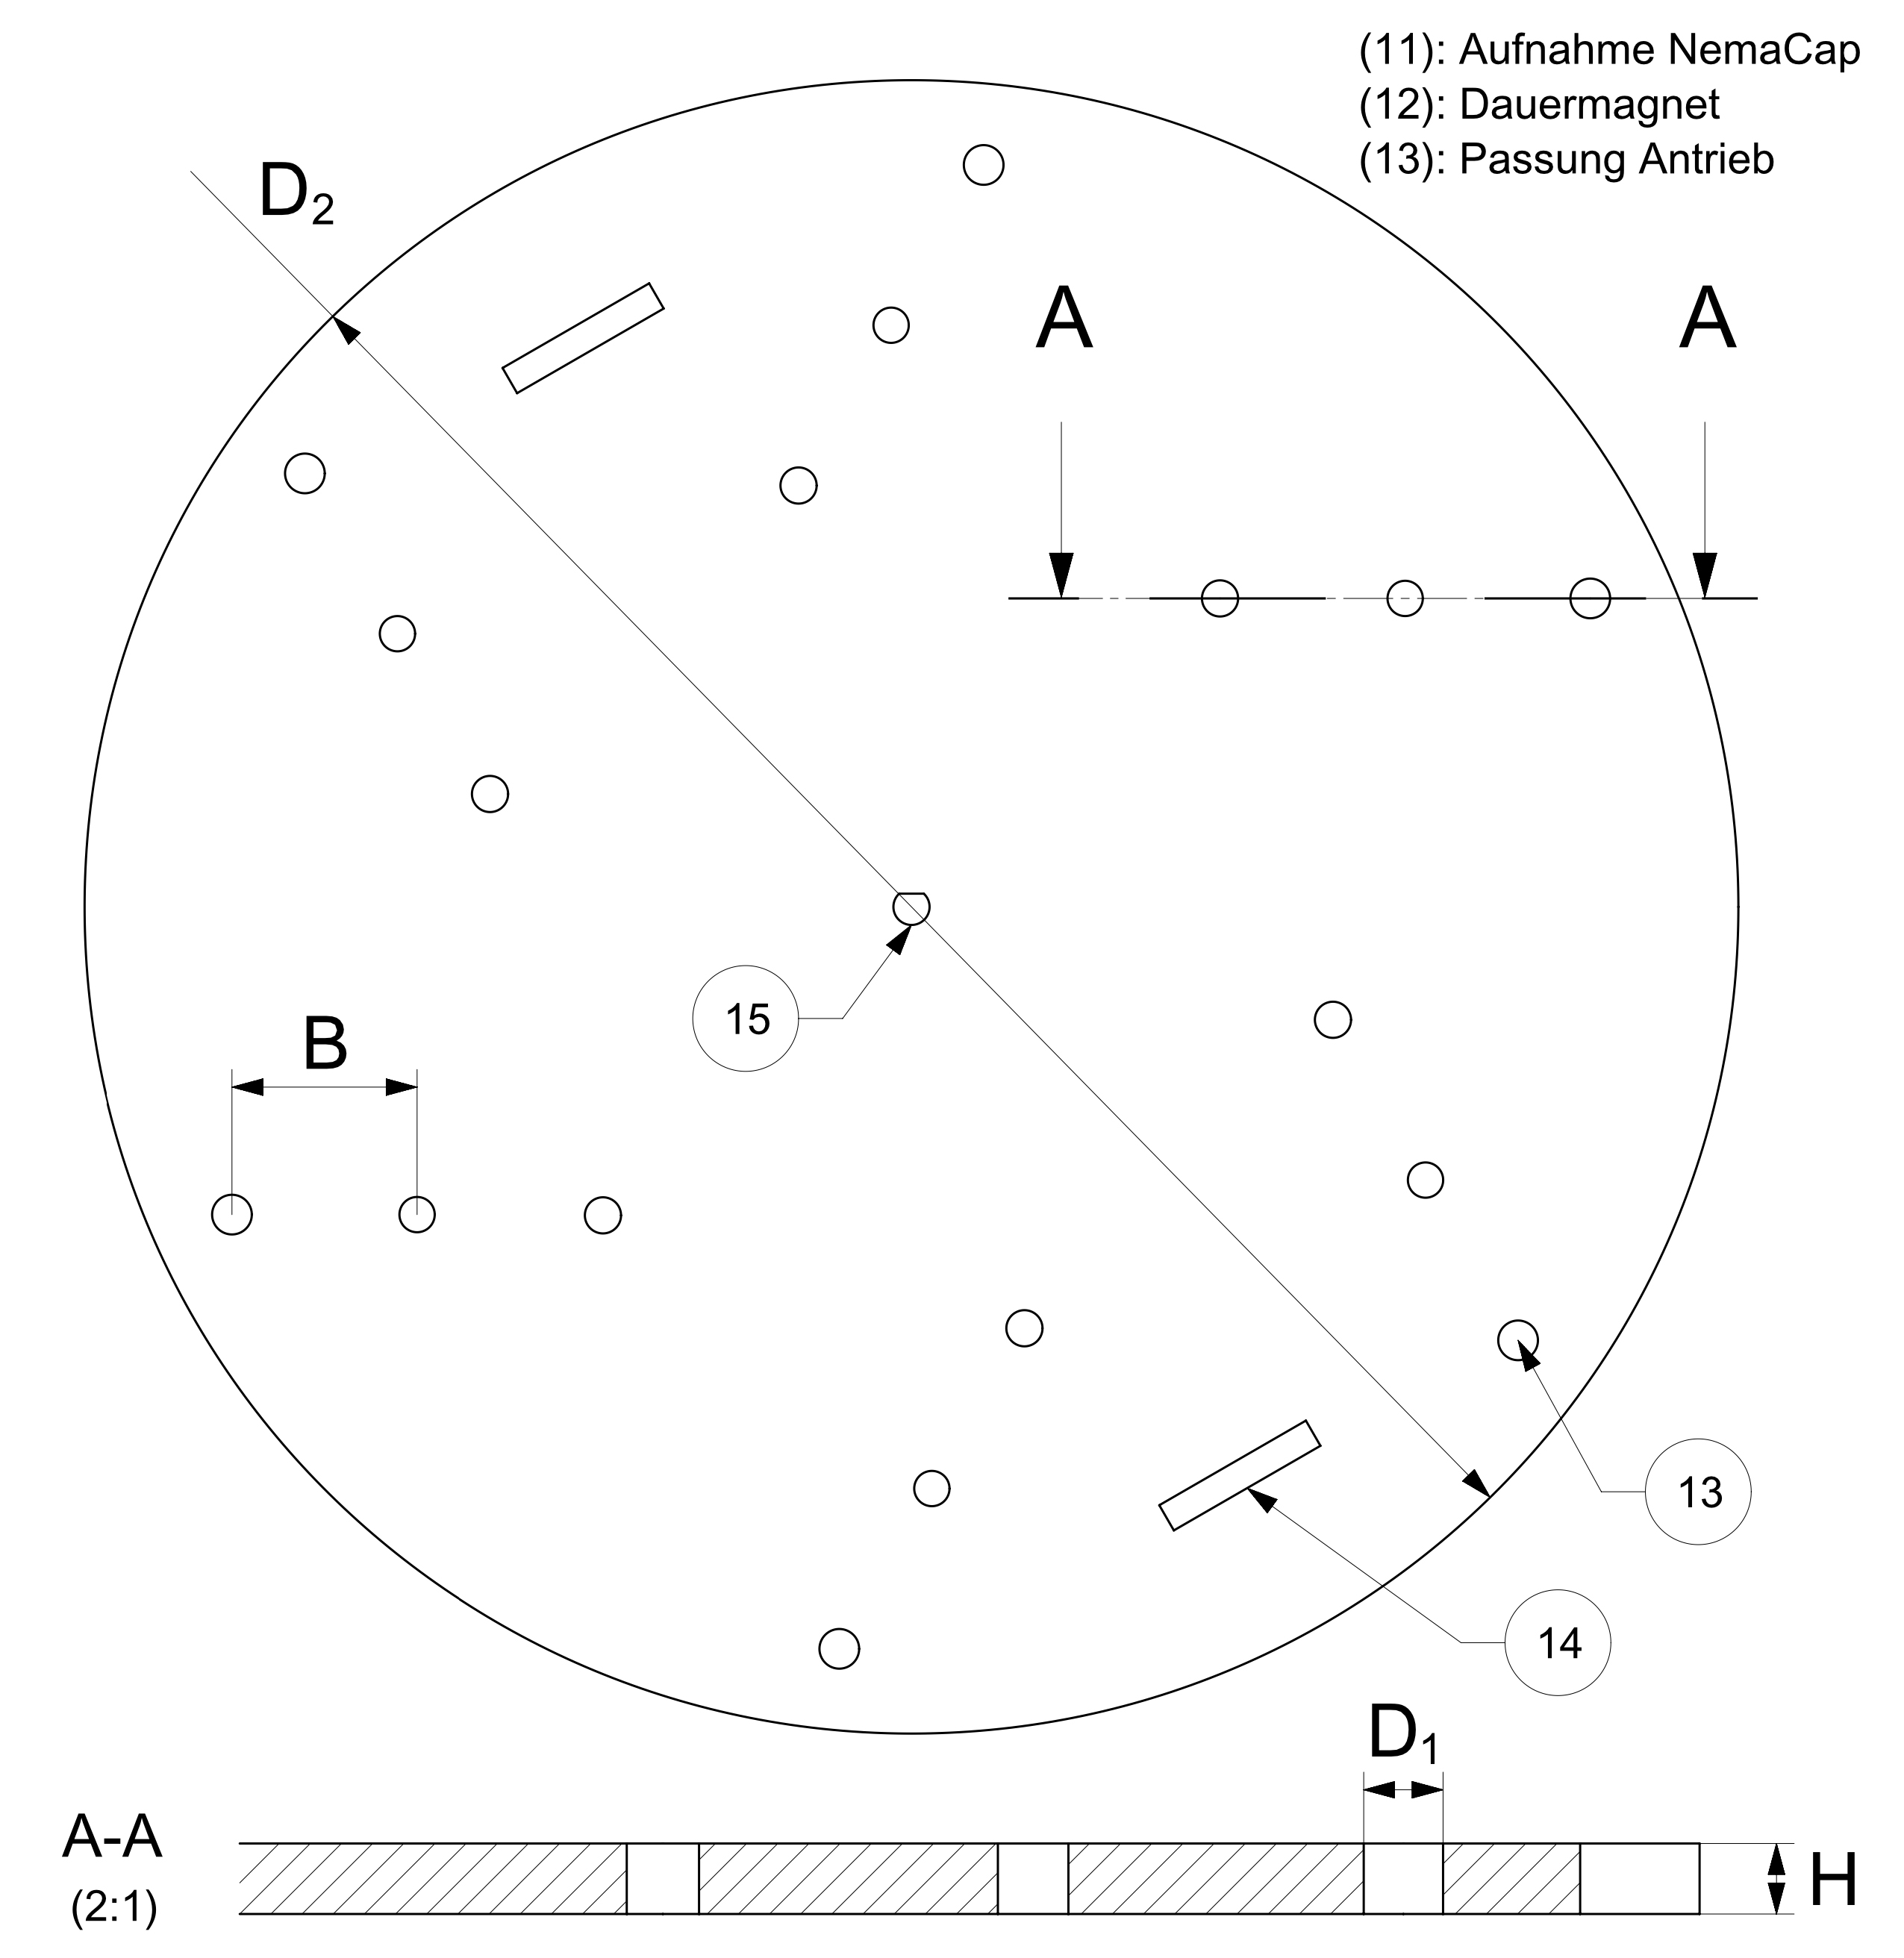
\includegraphics[scale=0.65]{Illustrationen/6-Umsetzung/detail_lochmaske.jpg}
	\caption{Grundriss der Lochmaske mit Schnitt}
	\label{fig:detail_lochmaske}
	\end{figure}
\textbf{Fertigungsverfahren und Materialwahl}
\newline
 Die Grundplatte sowie die Lochmaske werden mit dem Laser gefertigt. Dieses Fertigungsverfahren ist optimal für die Herstellung von zweidimensionalen Teilen. Ein Minimum von verschiedenen Blechdicken spart Umrüstungzeiten und senkt dadurch Kosten. Ein weiterer Vorteil ist, dass ein direkter Export der Fertigungsunterlagen aus dem CAD möglich ist. Für weitere Komponenten anderer Teilfunktionen wird die Realisation aus gelasertem Blech bevorzugt.
\newline
\newline
Die Vereinigung von verschiedensten Funktionen in der Trommel (Integralbauweise) führt zu einer komplexeren Geometrie. Fertigungstechnisch sind gewisse Geometrien konventionell nicht herstellbar. Daher bietet sich Rapid Prototyping als Fertigungsverfahren an. Dadurch ergibt sich jedoch eine Einschränkung: Der Aussendurchmesser der Trommel darf maximal 200mm betragen, da der Bauraum des internen 3D-Druckers 200mm x 200mm x 300mm beträgt. 